% USEFUL LINKS:
% -------------
%
% - UiO LaTeX guides:          https://www.mn.uio.no/ifi/tjenester/it/hjelp/latex/
% - Mathematics:               https://en.wikibooks.org/wiki/LaTeX/Mathematics
% - Physics:                   https://ctan.uib.no/macros/latex/contrib/physics/physics.pdf
% - Basics of Tikz:            https://en.wikibooks.org/wiki/LaTeX/PGF/Tikz
% - All the colors!            https://en.wikibooks.org/wiki/LaTeX/Colors
% - How to make tables:        https://en.wikibooks.org/wiki/LaTeX/Tables
% - Code listing styles:       https://en.wikibooks.org/wiki/LaTeX/Source_Code_Listings
% - \includegraphics           https://en.wikibooks.org/wiki/LaTeX/Importing_Graphics
% - Learn more about figures:  https://en.wikibooks.org/wiki/LaTeX/Floats,_Figures_and_Captions
% - Automagic bibliography:    https://en.wikibooks.org/wiki/LaTeX/Bibliography_Management  (this one is kinda difficult the first time)
%
%                              (This document is of class "revtex4-1", the REVTeX Guide explains how the class works)
%   REVTeX Guide:              http://www.physics.csbsju.edu/370/papers/Journal_Style_Manuals/auguide4-1.pdf
%
%
% COMPILING THE .pdf FILE IN THE LINUX TERMINAL
% ---------------------------------------------
%
% [terminal]$ pdflatex report_example.tex
%
% Run the command twice, always.
%
% When using references, footnotes, etc. you should run the following chain of commands:
%
% [terminal]$ pdflatex report_example.tex
% [terminal]$ bibtex report_example
% [terminal]$ pdflatex report_example.tex
% [terminal]$ pdflatex report_example.tex
%
% This series of commands can of course be gathered into a single-line command:
% [terminal]$ pdflatex report_example.tex && bibtex report_example.aux && pdflatex report_example.tex && pdflatex report_example.tex
%
% ----------------------------------------------------



\documentclass[english,notitlepage,reprint,nofootinbib]{revtex4-1}  % defines the basic parameters of the document
% If you want a single-column, remove "reprint"

% Allows special characters (including æøå)
\usepackage[utf8]{inputenc}
% \usepackage[english]{babel}

% Note that you may need to download some of these packages manually, it depends on your setup.
% It may be usefult to download TeXMaker, because it includes a large library of the most common packages.

\usepackage{physics,amssymb}  % mathematical symbols (physics imports amsmath)
\include{amsmath}
\usepackage{graphicx}         % include graphics such as plots
\usepackage{xcolor}           % set colors
\usepackage{hyperref}         % automagic cross-referencing
\usepackage{listings}         % display code
\usepackage{subfigure}        % imports a lot of cool and useful figure commands
% \usepackage{float}
%\usepackage[section]{placeins}
\usepackage{algorithm}
\usepackage{placeins}
\usepackage[noend]{algpseudocode}
\usepackage{subfigure}
\usepackage{comment}
\usepackage{tikz}
\usetikzlibrary{quantikz}
% defines the color of hyperref objects
% Blending two colors:  blue!80!black  =  80% blue and 20% black
\hypersetup{ % this is just my personal choice, feel free to change things
    colorlinks,
    linkcolor={red!50!black},
    citecolor={blue!50!black},
    urlcolor={blue!80!black}}


% ===========================================


\begin{document}

\title{Numerical solution of 2D Ising model}  % self-explanatory
\author{Lukas Cernusak} % self-explanatory
\date{November 2023}                             % self-explanatory
\noaffiliation                            % ignore this, but keep it.

%This is how we create an abstract section.

\begin{abstract}

We are solving numerically 2D Ising model with periodic boundary conditions, using Marco chain Monte Carlo and Metropolis algorithms in the canonical ensemble. A solution of a two-by-two lattice is compared to the analytical result, exploiting error. A twenty-by-twenty solution is used to find burn-in time, which is determined to be about $2000$ Monte Carlo cycles. A conditional probability mass function $p(\epsilon; T)$ is sampled for the same lattice size with temperature $1J/k_B$ and $2.4J/k_B$ and the variance turns out to be two orders of magnitude smaller for the low energy function. An estimate of critical temperature for an infinite lattice is determined to be $2.273 \pm 0.008 J/k_B$.

\end{abstract}



\maketitle







% ===========================================
\section{Introduction}
%
Magnets are everywhere. Their application is extremely broad, all the way from cheap fridge-badge to particle super colliders. The spectrum of possible technologies, that could be made possible using for instance superconductors is immense. It is therefore not a surprise the research regarding them is vivid to say at least. As proof, we may regard the hot headlines about the LK-99 room-temperature superconductor, which although on the unclear ground, made it to science news all around the world. The strongest interacting, and possibly the best known, type of magnet is a ferromagnet. In this report, we will work with a ferromagnetic model, namely the Ising model.

The Lenz-Ising model, dating back to 1920, is named after Ernst Ising, who solved analytically the 1D problem, and Wilhelm Lenz, who created it. It models a ferromagnet as a number of interacting spins, which may take on two values, either up or down. 

In comparison to the 1D model, the 2D model undergoes a phase transition at a critical temperature $T_C$. Lars Onsager was the first person to solve the infinite 2D Ising model analytically and determine its critical temperature. The ultimate goal of this report is to estimate the same value.

The model is in a canonical ensemble, meaning the probabilities of spin configurations, are given by Boltzmann statistics. Of course, it is possible to determine the exact solutions for lattices with finite number of spins, but this would require us to find the partition function, which scales with the total number of possible states, meaning it is quite unpractical for large lattices. Instead, it is possible to simulate the evolution of the model, which only requires relative probabilities between states.

To find the evolution of the system, we will use the Marco chain Monte Carlo method (MCMC), together with the Metropolis algorithm. Our model will be in a crystal square structure (lattice) and it will have periodic boundary conditions. This means, in reality, we are working with a Torus. 

The simple two-by-two lattice will be solved analytically too, such that it is possible to compare the numerical result to it and test our implementation. Furthermore, we will exploit the burn-in time, which physically corresponds to the time needed to reach equilibrium, starting from an initial configuration. Also, we will sample and approximate a conditional probability mass function for energy. Ultimately, we will determine the critical temperature for four different lattice sizes, and use the result to estimate the temperature for an infinite lattice.












% ===========================================
\section{Methods}\label{sec:methods}
%
\subsection{General}\label{sec:General}

Our model is a square lattice, organized in a square crystal structure, with periodic boundary conditions and with the same number of spins $L$ along both axes. The total number of spins is given as $L \cdot L = N$. These spins may take on values $\pm1$, representing spins up ($1$) and spin down ($-1$). This obviously corresponds to the famous quantum mechanical property of spin $\frac{1}{2}$ particles. Such a lattice may be represented using a vector $\vec{s} = (s_1, s_2, \cdot \cdot \cdot, s_N)$, where $s_i$ corresponds to the orientation of ith spin. Note that unless in the presence of a magnetic field, due to rotational symmetry, the model will not differentiate between up and down orientation, meaning $\vec{s}$ will have identical properties as $ - \vec{s}$.

We will be working in the canonical ensemble, meaning the system is allowed to exchange temperature with the surroundings, which acts like a heat reservoir with an infinite heat capacity. In this ensemble, given a temperature $T$, we may calculate the probability of a system to be in a state with energy $E(\vec{s})$, using Boltzmann factor and partition function $Z$, as
\begin{equation}
    p(\vec{s};T) = \frac{1}{Z} e^{- \beta E(\vec{s})}.
\end{equation}
The variable beta is simply $\beta = \frac{1}{T k_B}$, where $k_B$ is the Boltzmann's constant. The partition function corresponds to the stochastic normalization requirement and is computed as
\begin{equation}
    Z = \sum_{\text{all } \vec{s}} e^{- \beta E(\vec{s})}.
\end{equation}

There are two intrinsic values we may measure given a state $\vec{s}$, magnetization, and energy. The total energy of the system will be denoted using capital $E$, and energy per particle using lowercase $\epsilon$. These are defined as
\begin{equation}
    E(\vec{s}) = -J \sum _{\langle k,l \rangle} ^N s_k s_l
\end{equation}
\begin{equation}
    \epsilon (\vec{s}) = \frac{E(\vec{s})}{N} .
\end{equation}
Here $\langle k,l \rangle$ denotes neighboring spins without double counting. Note that $\epsilon$ is a macroscopic value corresponding to an average energy per spin, not a microscopic one. The letter $J$ represents the coupling constant which shall always be positive. A justification for this is provided by the third law of thermodynamics, which states that the entropy needs to approach a minimum as temperature goes to zero. This requires the model to take on an ordered structure, where all spins will have the same orientation. Simultaneously the Boltzman statistics specify that the state with the lowest energy will be the only possible one as the temperature goes to zero. Combining these two arguments means the coupling constant needs to be positive, such that the ordered system has the lowest possible energy. This is of course backed by experimental results, as ferromagnets do exhibit such behavior.

The next variable we take interest in is the magnetization. In comparison to energy, magnetization is a vector quantity, which in our system can either take a positive or negative value. Here I recall the argument about rotational symmetry, making the sign ambiguous and we shall therefore measure only the absolute value of the magnetization. Just as with energy,  we will measure two macroscopic values, the total magnetization denoted by capital $M$ and the average magnetization per particle $m$. These may be found using
\begin{equation}
    |M(\vec{s})| = \Big|\sum_i ^N s_i \Big|
\end{equation}
\begin{equation}
    |m(\vec{s})| = \frac{|M(\vec{s})|}{N}.
\end{equation}


 Technically, we now have all we need to solve the Ising model analytically. However, for large lattices, this would be difficult, because as the lattice grows, there are more possible states, and the partition function keeps expanding. Therefore we will be solving problems numerically, but we still would like to verify at least some of our approaches to analytical solutions. To do so, we will use the smallest non-trivial lattice, the two-by-two.

\subsection{Two-by-two}
 
 We start off by finding all possible states of such a lattice. Imposing rotational symmetry, it turns out there are six different states the model can be in. In table \ref{table:1} there is an overview of them, with values for the up-oriented spins, denoted $\uparrow$, the total energy of the system $E$, net magnetization $|M|$ and degeneracy $g$.


\begin{table}[h!]
\centering
\begin{tabular}{||c c c c||} 
 \hline
  $\uparrow$ & $E[J]$ & $|M|$ & $g$ \\ [0.5ex] 
 \hline\hline
 0 & -8 & 4 & 1 \\ 
 1 & 0 & 2 & 4 \\
 2 & 0 & 0 & 4 \\
 2 & 8 & 0 & 2 \\
 3 & 0 & 2 & 4 \\ 
 4 & -8 & 4 & 1 \\ [1ex] 
 \hline
\end{tabular}
\caption{Table gives associated values for non-identical states in a two-by-two lattice. Energy is measured using the coupling constant $J$.}
\label{table:1}
\end{table}


There are two different states both with the same number of spins oriented up and down. The first is trans-state, where the equality-oriented spins are neighbors, and cis-states, where they are not. Here we may clearly observe a result of the rotational symmetry argument, as states that are inverse of each other have the same energy. Really, there should only be four states in this table, and the value for the number of spin-up states should be neglected altogether.

We will calculate four values, which we will later compare with those obtained numerically. These will be the expectation values of energy per particle $\rangle  \epsilon \langle$, the expectation value of the magnetization per particle $\langle | m | \rangle$, the heat capacity per particle $c_V$ and the magnetic susceptibility per particle $\chi$. However, to find the $c_V$ and $\chi$ we will need to know the variance of $\epsilon$ and $m$, so we need to find values for $\rangle  \epsilon ^2 \langle$ and $\langle | m |^2 \rangle$ too. Using the standard equation $\langle Q \rangle = \sum Q \cdot p(Q) $, where $Q$ is an arbitrary variable, and $p(Q)$ is a probability mass function for value Q, gives us 
\begin{equation} \label{eq:7}
    \langle \epsilon \rangle = \frac{1}{Z} \sum_{i=1} ^{16} \frac{E_i}{N} e^{- \beta E_i} = - \frac{32J}{ZN} sinh(8 \beta J)
\end{equation}
\begin{equation}
    \langle \epsilon ^2 \rangle = \frac{1}{Z} \sum_{i=1} ^{16} \Big( \frac{E_i}{N} \Big)^2 e^{- \beta E_i} = \frac{256J^2}{ZN^2} sinh(8 \beta J)
\end{equation}
\begin{equation}
    \langle |m| \rangle = \frac{1}{Z} \sum_{i=1} ^{16} \frac{|M_i|}{N} e^{- \beta E_i} = \frac{8}{ZN}  (2 + e^{8 \beta J})
\end{equation}
\begin{equation}
    \langle |m| ^2 \rangle = \frac{1}{Z} \sum_{i=1} ^{16} \Big( \frac{|M_i|}{N} \Big)^2 e^{- \beta E_i} = \frac{32}{ZN^2} (1 + e^{8\beta J}).
\end{equation}

Now we may deduce the heat capacity and magnetic susceptibility. As variance may be expressed using expectation values $Var(Q) = \langle Q^2 \rangle - \langle Q \rangle ^2$ we have that
\begin{equation}
    c_V = \frac{1}{k_B T^2 N} (\langle \epsilon ^2 \rangle - \langle \epsilon \rangle ^2)
\end{equation}
\begin{equation}\label{eq:12}
    \chi = \frac{1}{k_B T N} (\langle |m|^2 \rangle - \langle |m| \rangle ^2).
\end{equation}






\subsection{Phase transition}

  In 1936 Rudolf Peierls proved that the 2D Ising model, undergoes a phase change from an order ferromagnetic to a disordered state at some critical temperature $T_C$. An analytical value for this temperature was first given by Lars Onsager in 1944, and it reads $T_C(L=\infty) \approx 2.296 J/k_B $. The critical behavior is described by power laws, where in the case of the 2D Ising model we have
\begin{equation}
    \langle |m| \rangle \propto |T - T_C(L=\infty)|^\beta
\end{equation}
\begin{equation}
    C_V \propto |T - T_C(L=\infty)|^{- \alpha}
\end{equation}
\begin{equation}
    X \propto |T - T_C(L=\infty)|^{- \gamma}.
\end{equation}
\begin{equation} \label{eq:16}
    \xi \propto |T - T_C(L=\infty)|^{- \nu}.
\end{equation}
Here the exponents are so-called \textit{critical exponants}, and capital $C_V$ and $X$ are respectively the thermal capacity and magnetic susceptibility of the whole lattice. The variable $\xi$ is called \textit{correlation lengdth} and corresponds to the typical length scale of regions with aligned spins. For temperatures near $T_C$ the critical exponents are $\beta = \frac{1}{8}$, $\alpha = 0$,  $\gamma = \frac{7}{4}$ and $\nu = 1$. 

Both $C_V$ and $X$ diverge for $T=T_C$, which is the principle we will use to decide what the critical temperatures are, based on numerical results, but let's not get ahead of ourselves. The correlation length $\xi$ also diverges at critical temperature, but as we are working with finite lattices, the largest value it can take is L. If we introduce a proportionality constant $a$ and rewrite the \ref{eq:16}, we arrive to
\begin{equation} \label{eq:17}
    T_C(L) - T_C(L=\infty) = aL^{-1}.
\end{equation}
This equation allows us to determine $T_C(L \rightarrow \inft)$, using for instance linear regression with a few finite samples computed numerically.



\subsection{Algorithms}

Using the Boltzmann statistics, we may define a conditional probability mass function $p(\vec{s}; T)$, which returns a probability of any given macrostate $\vec{s}$. This function has $N$ dimensions, where each variable has a domain $\{-1,1\}$. As mentioned before, the partition function makes it difficult to find the exact solution. What we therefore wish to do instead, is to sample this probability distribution using a Monte Carlo method.
Generally, \textit{Monte Carlo} describes methods that use random numbers to operate. Some possibilities interesting for us include rejection sampling or inverse transform sampling. Unfortunately, rejection sampling works poorly with high dimensional distributions, and inverse sampling would require us to know the partition function, the absence of which is the primary motivation for the numerical approach.
The approach we will use is known as the \textit{Marco chain Monte Carlo} (MCMC for short). This method works well in high-dimensional space, as it essentially is just a walker with bias motion. Some drawbacks of this sampling method, include the limited capability of overcoming regions with low probability, or a high correlation between individual steps. 
As the peaks of the probability functions are generally unknown, initializing the MCMC from a random position, may cause the results to become biased, as the walker may spawn at an otherwise unlikely position. This phenomenon is usually referred to as \textit{burn-in} and may be overcome by discarding a number of initial steps.
For implementing the MCMC, we need to take into account two processes. 
(i) A step needs to be proposed. Since in in our case the domain of all variables only consists of two elements, the proposal is limited to the opposite of the current state. As in our case, there is no reason for bias propositions, we will use a uniform probability mass function (pmf), as our proposal probability $T(s_i \rightarrow -s_i) = \frac{1}{N}$. 
(ii) A step needs to be accepted. We need an acceptance pmf $A$ defining the probability of accepting the proposed state. That requires an algorithm that fulfills both the detailed balance and ergodicity, ensuring the results will converge to the analytical solutions for an infinite number of steps. The pmf in Metropolis algorithm is given as
\begin{equation}
    A(s_i \rightarrow -s_i) = min \Big( 1, \frac{p(-s_i)}{p(s_i)} \frac{T(-s_i \rightarrow s_i)}{T(s_i \rightarrow -s_i)} \Big)
\end{equation}
Here $p(s_i)$ is the probability of state $s_i$. Notice that the algorithm only depends on the relative difference between the probabilities, which can be easily found using Boltzmann factors without the need for a partition function. Furthermore, since we chose $T$ to be uniform, the relation between the proposal probabilities will always be one and we may disregard it. 
The actual decision of whether a proposal will be accepted or not, will be made by comparing the acceptance probability to a random number drawn from a uniform distribution. Setting this together, and substituting $p$ with Boltzmann's factors, gives us that the proposed state will be accepted iff one of the following is true
\begin{equation}
    \Delta E < 0
\end{equation}
\begin{equation}
    \Delta E > 0 \text{ and } e^{-\beta \delta E} \geq r.
\end{equation}
Here $r$ is a random number between $0$ and $1$ drawn from a uniform distribution, and the energy difference corresponds to $\Delta E = E_{\text{after}} - E_{\text{before}}$. The last thing to mention is that the algorithm only converges to the correct solutions, and in addition to burn-in time, there will also be an associated statistical uncertainty.









\subsection{Tools}
A central tool for all our simulations is a random number generator (RNG for short). First of all, while saying random numbers, what we really mean is pseudorandom numbers. The difference is that pseudorandom numbers are possible to predict, as they are elements of some sequence. There are two basic things to consider while comparing the quality of an RNG, firstly the period, which corresponds to the length of the sequence before it starts to repeat itself, and whether the numbers trually are distributed evenly in a uniform distribution, with minimal correlations. In our simulations, we will use RNG called \textit{Mersenne Twister MT-19937} from C++. standard library. This RNG, as the name suggests, has a period of $2^{19937}$ numbers.
Now more generally about other tools that have been used. One loop in the code has been parallelized using OpenMP. The C++ Chrono function was used to measure the duration of different runs. Further, we have used matrices and random function `randu` from the C++ armadillo library. All plots have been made using Pythons matplotlib in cooperation with numpy.

\subsection{Code}
Unfortunately, I haven't managed to paralyze the code using Open MP, as although the code worked as desired, no increase in computational speed was observed. I ended up using the "dummy paralyzation" and ran the code for different lattice sizes simultaneously. On the other hand, adding the \textit{-O3} flag improved the speed significantly.
In order to avoid some unnecessary calculations, it can be easily proven that a spin flip can be associated with only five different changes in the energy, namely $\Delta E \in \{ -16,-8,0,8,16\}[J]$. Furthermore, only for two of these cases is it necessary to calculate the acceptance probability, as three of them are smaller or equal to zero. The code constructor precalculates these two factors. Simultaneously, to avoid costly \textit{if} test, there is an indexing vector that makes it possible to enforce the boundary conditions without any tests.
On the other hand, there are multiple highly inefficient processes in the code. For instance, data that are often not needed for particular simulations are often computed and stored, or parts of the expectation values are recalculated although they could relatively easily be reused to update the new expectation value.


\subsection{Simulation}
Firstly, we will run a simulation of a two-by-two-by lattice. The main purpose is to validate our numerical approach by comparing expectation values, $c_V$, and $\xi$ (values of interest) with analytical solutions. The simulation has $10^6$ points per temperature, burn-in is $10$ steps, and every Monte Carlo (MC) cycle, corresponding to every 4th step, will be saved. The temperature range is $T \in [1,5] J/k_B$, with $20$ temperature steps. The initial configuration is disordered and is determined by armadillo's \textit{randu} function with seed $123$. This seed will be the benchmark for all disordered systems. There is also an option to run randomly generated seeds determined by the system clock.

Second, we wish to study the error in the two-by-two cases. There will be two different simulations, again with $L=2$, for temperatures of $1.0 J/k_B$ and $2.4 J/k_B$ and starting from a disordered state. As it is the error we wish to explore, there are no burn-in steps, and every MC cycle is saved. The simulation makes $4000$ steps corresponding to $1000$ MC cycles per temperature.

The objective of the third simulation is to study the burn-in time. This requires a larger lattice, so we use $L=20$. There are in total four individual simulations, with temperatures $1.0 J/k_B$ and $2.4 J/k_B$ and starting from both ordered and disordered states. Of course, there are no burn-in steps and each simulation runs $2000$ MC cycles.
Values the code saves are always computed from the whole available interval. This has an effect of seemingly extending the burn-in time, as the values from before equilibrium was reached will always be present.

The purpose of the fourth simulation is to estimate the energy pmf $p(\epsilon ; T)$. The lattice size and temperatures stay unchanged. The initial state will be disordered, with $2000$ burn-in MC cycles and a total of $10^8$ steps. Every MC cycle will be stored. In comparison to the simulations above, here we are not interested in the values of interest, but rather the individual energy and magnetization measurements themselves.

Finally, the fourth simulation will attempt to map the values of interest in proximity to the critical temperature. The temperature will be $T 
\in [2.1,2.4] J/k_B$. There will be for lattice sizes, $L=40,60,80,100$. Each lattice will run for $100$ different temperatures, with $10^9$ steps per temperature, and every MC cycle will be stored. The burn-in time for all will be $2000$ MC cycles, and $10$ MC cycles to reach equilibrium after a temperature change, which should be sufficient, as the end of one simulation with some temperature will be the initial state for the next simulation with only slightly higher temperature.

























% ===========================================
\section{Results and discussion}\label{sec:results_and_discussion}
%


\subsection{The two by two}

To benchmark the numerical approach we compare the analytical solutions obtained from equations (\ref{eq:7}) and (\ref{eq:12}) to the numerical results. Graph for the value of interest is given in Figure \ref{fig:4b}. We see a close correlation between the values, indicating that we have implemented the algorithm correctly.  


\begin{figure}[h!]
    \centering %Centers the figure
    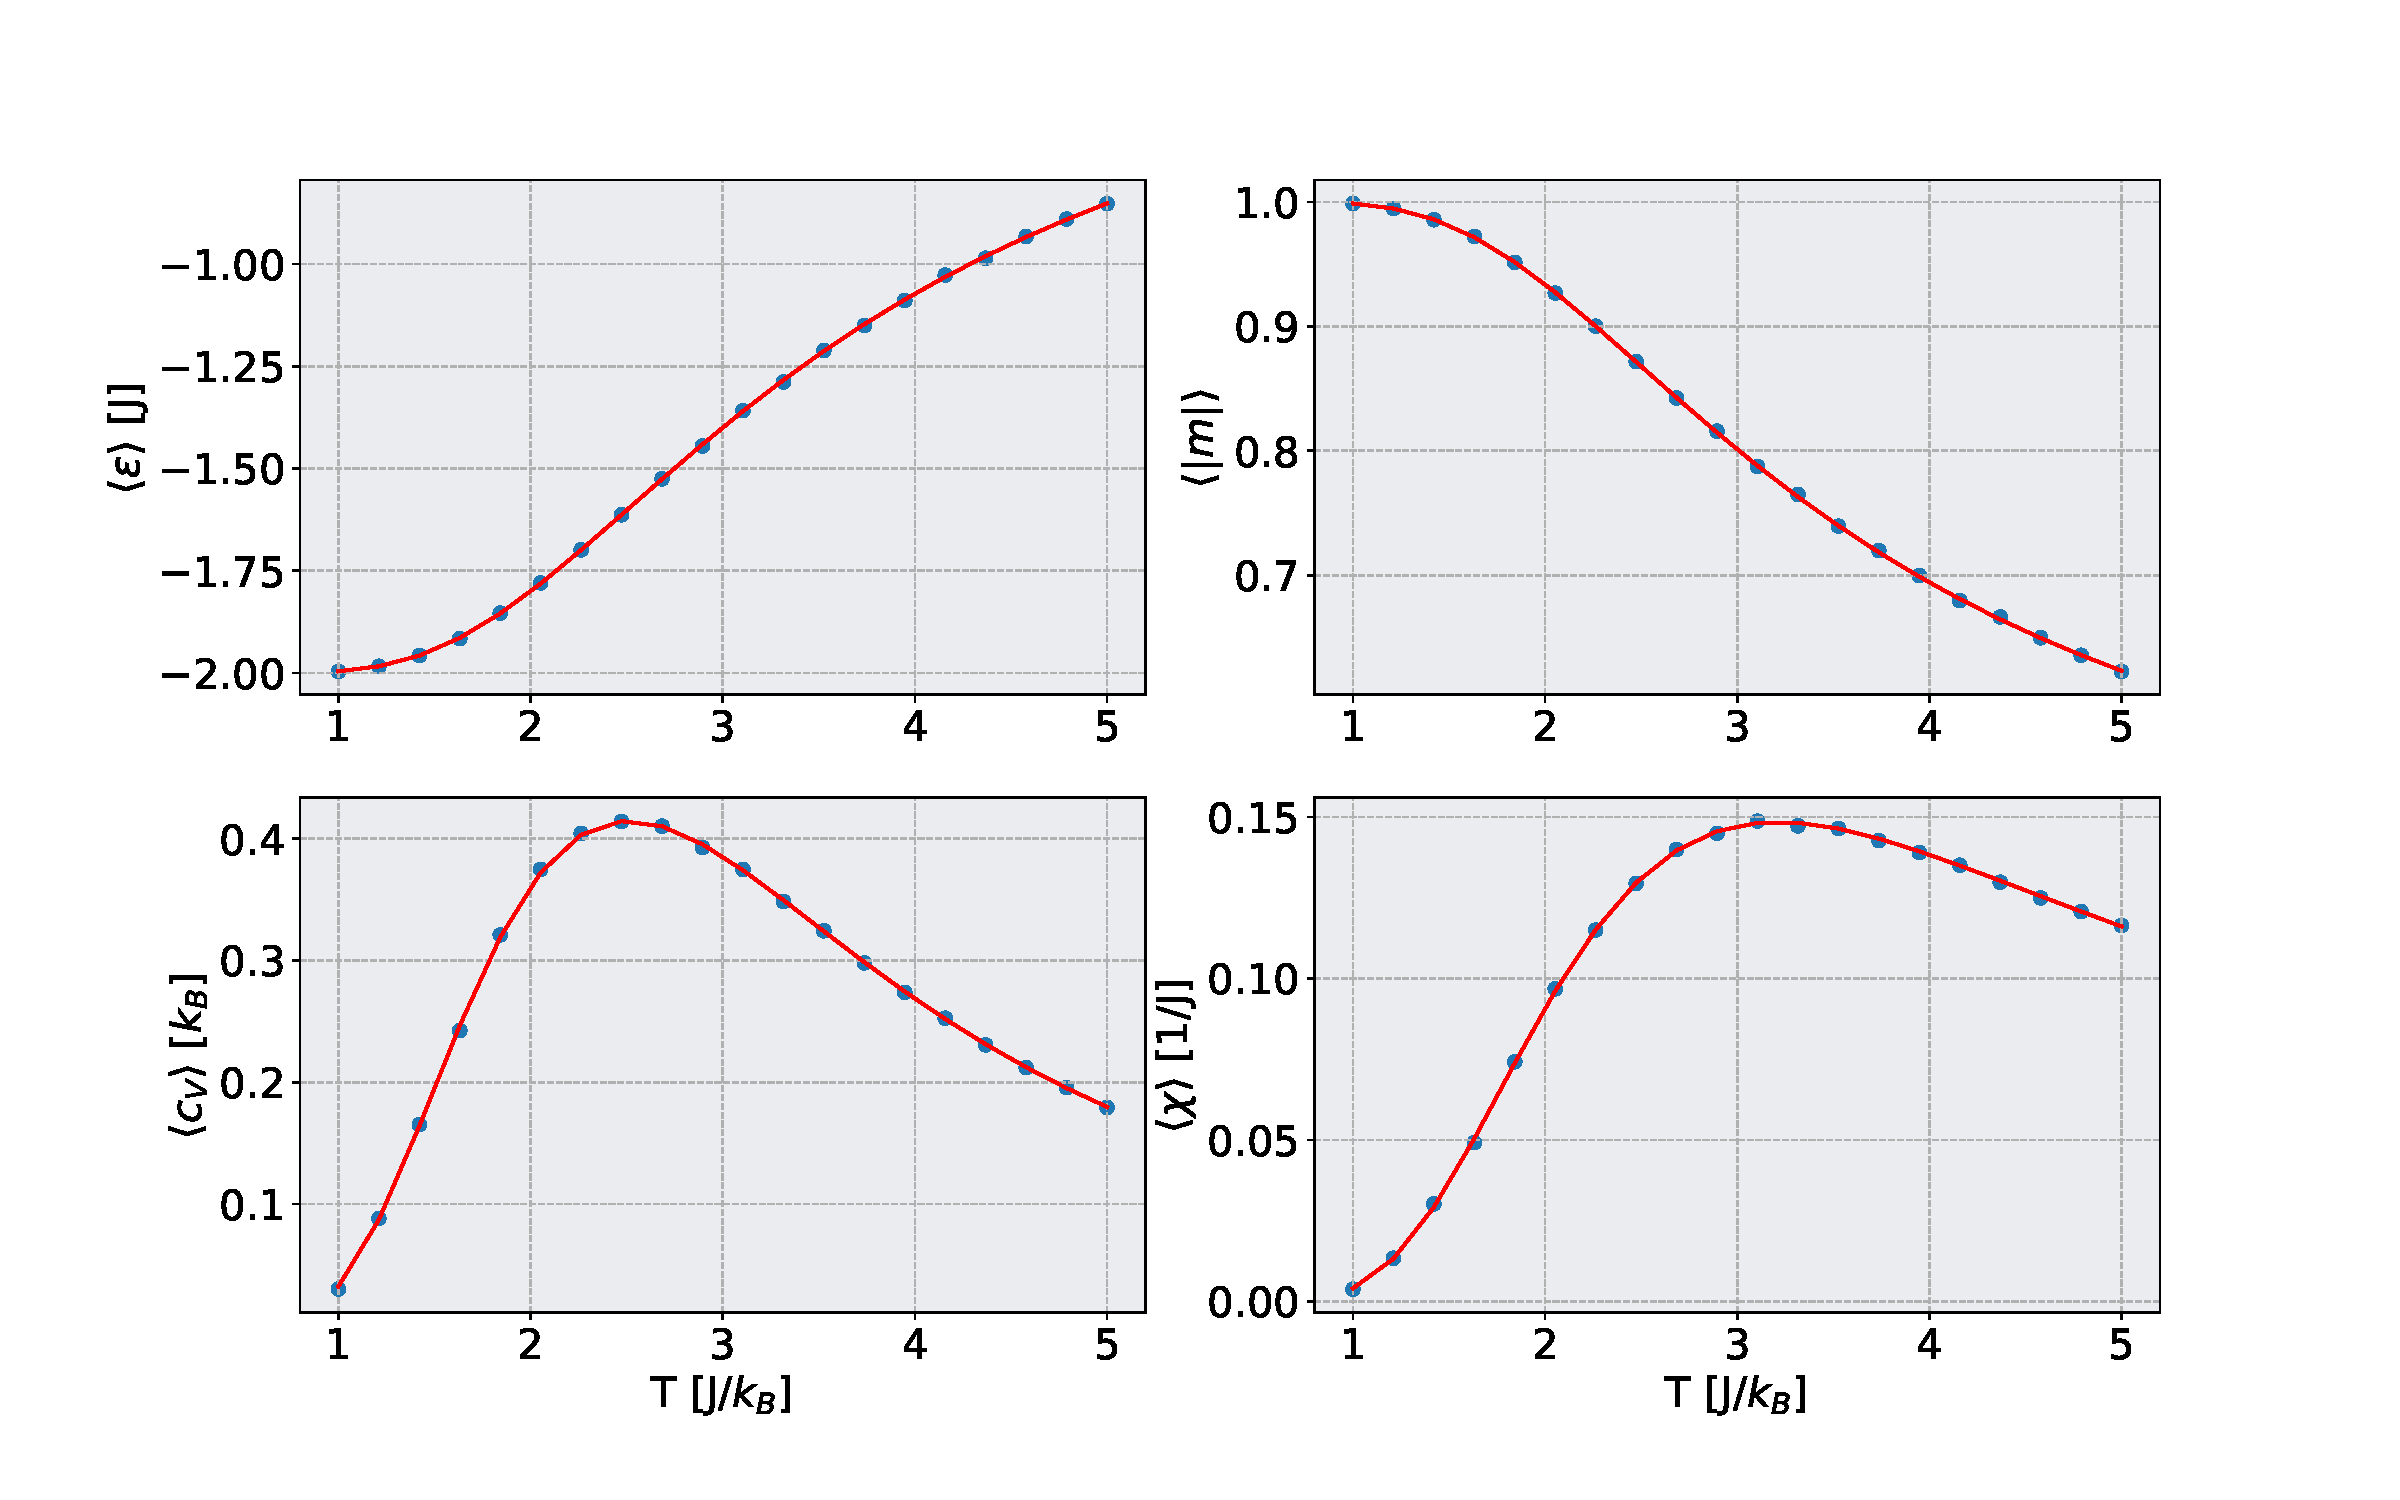
\includegraphics[scale=0.2]{figures/4b.pdf} %Imports the figure.
    \caption{Plot of values obtained for a 2x2 lattice, blue dots are numerical results, red lines are analytical solutions.}
    \label{fig:4b}
\end{figure}


As we now know the simulation is working as desired, we may exploit the error made by the method. Note that while computing the values of interest for a two-by-two lattice, the burn-in time is much smaller than the statistical uncertainty. Figure \ref{fig:4c} visualizes the absolute error on a logarithmic scale. The error seems to converge for the lower temperature and fluctuate for the higher temperature. However, for enough steps, the higher temperature would certainly converge too. It may be beneficial to plot this plot for a higher number of MC cycles.



\begin{figure}[h!]
    \centering %Centers the figure
    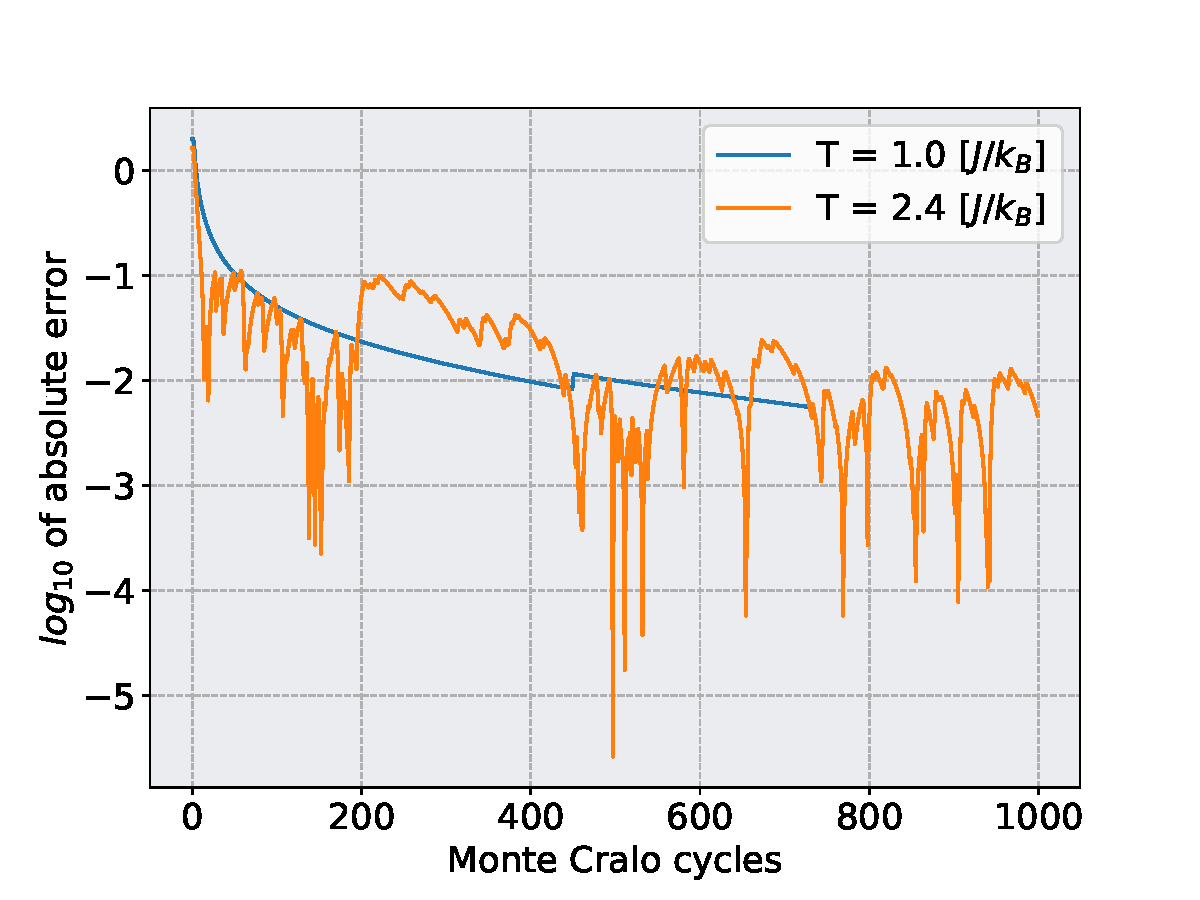
\includegraphics[scale=0.35]{figures/4c.pdf} %Imports the figure.
    \caption{Plot on logarithmic scale base of absolute error on a 2x2 lattice as a function of MC samples.}
    \label{fig:4c}
\end{figure}


\subsection{Tweny by twenty}

Now we wish to estimate the burn-in time. A plot of the expectation value for energy and magnetization as a function of MC cycles is provided in figure \ref{fig:5}. The two temperatures have vastly different properties. The higher temperature again seems to be fluctuating and the lower seems to converge. Intuitively, this makes sense as the random configuration is a more energetic state, than the equilibrium for both of the temperatures. It is therefore expected that there will be a bias in heat flow outside the lattice, which is clearly the case for both temperatures. However, the high-energy nature allows for more statistical uncertainty than the low temperature, which will converge to equilibrium at rates proportional to the energy difference. Of course, as we are working with finite lattices, the low-energy lattice is guaranteed to reach equilibrium in a finite number of steps. From these graphs, it seems like an acceptable burn-in time is around $2000$ MC cycles. 


\begin{figure}[h!]
    \centering %Centers the figure
    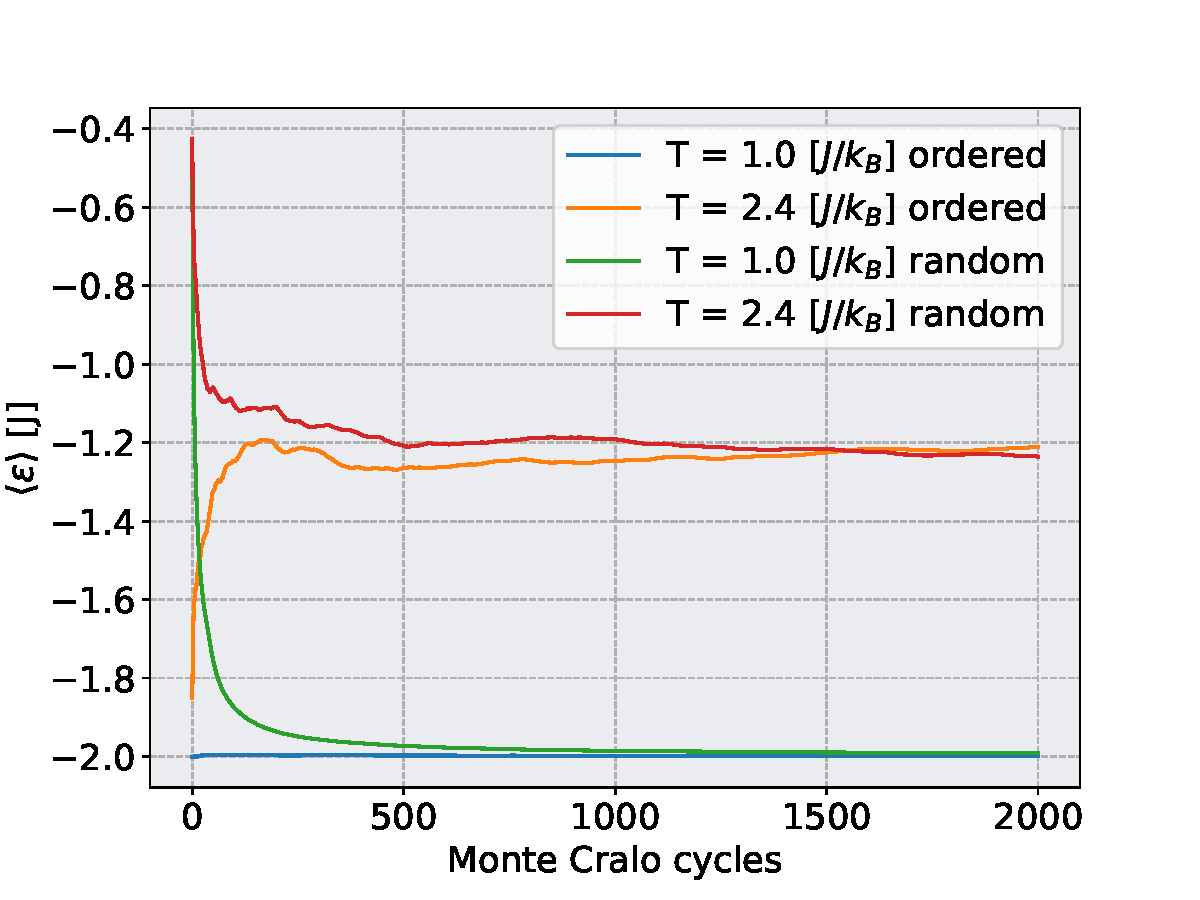
\includegraphics[scale=0.4]{figures/5e.pdf} %Imports the figure.
    \label{fig:5}
\end{figure}


\begin{figure}[h!]
    \centering %Centers the figure
    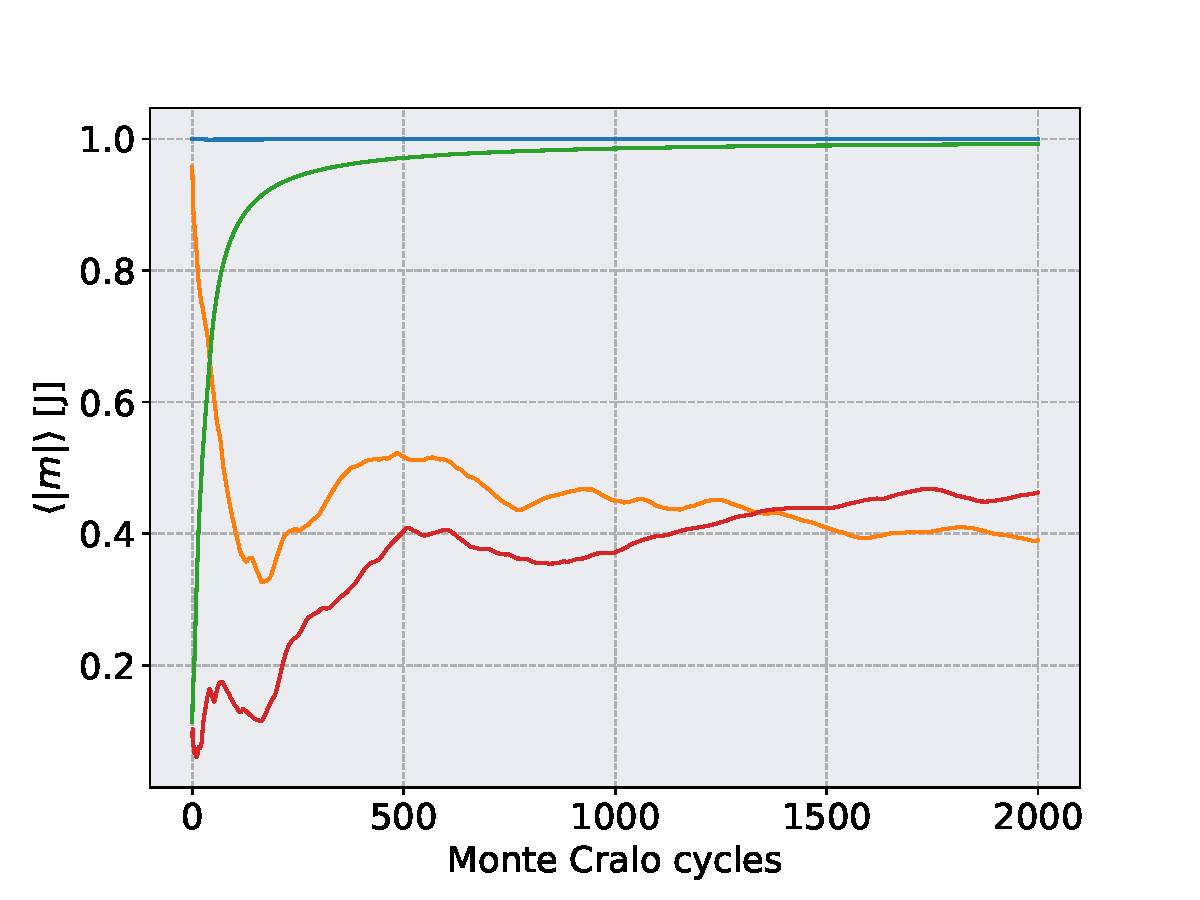
\includegraphics[scale=0.4]{figures/5m.pdf} %Imports the figure.
    \caption{Plot of the expectation value of energy and magnetization, as a function of MC cycles. The simulation is for a 20x20 lattice, starting from two different temperatures and both ordered and random initial states.}
    \label{fig:5m}
\end{figure}


The next simulation is for approximating the $p(\epsilon; T)$ function. A histogram with 100 bins for the higher temperature and 50 bind for the lower temperature can be seen in figure \ref{fig:6}. The variance in the lower temperature is $0.000197J^2$ and $0.0196J^2$ for the higher one. The pattern isn't surprising considering the ferromagnetic properties of the model. Decreasing probability for higher energy states while the temperature is low and vice versa is exactly what is intuitive. The higher temperature closely resembles a parabola, which is a sign that the probability distribution is normal.

\begin{figure}[h!]
    \centering %Centers the figure
    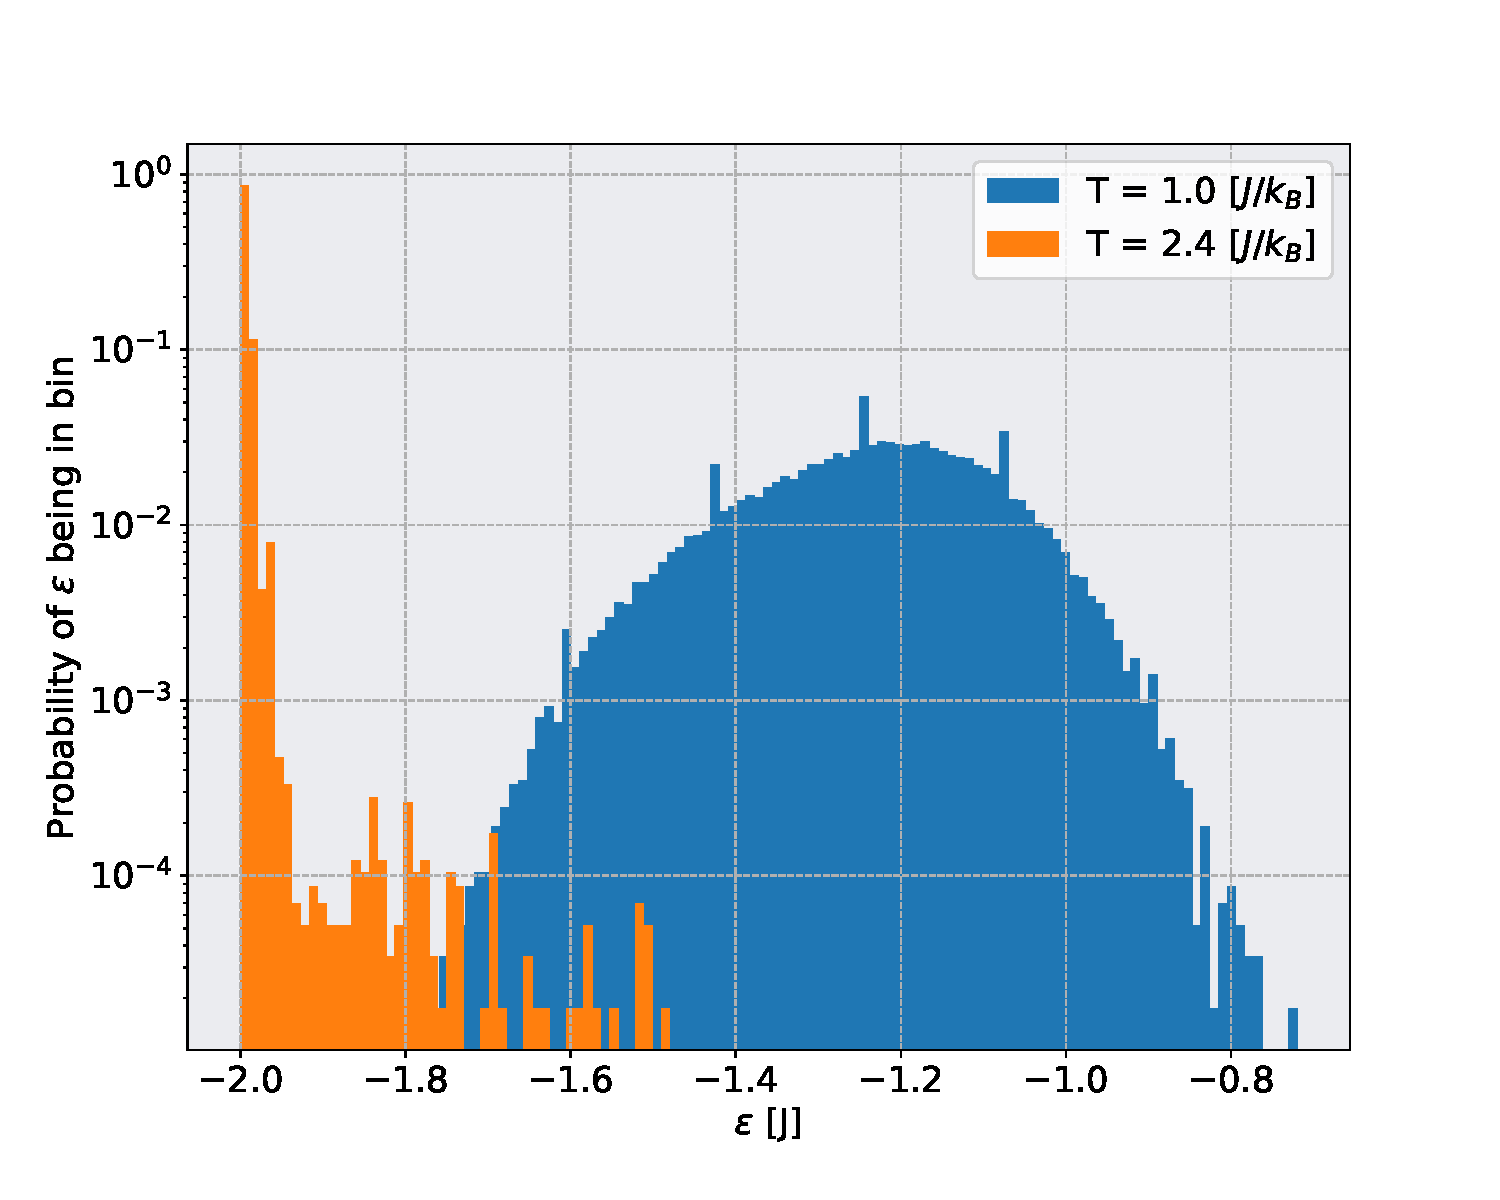
\includegraphics[scale=0.35]{figures/6.pdf} %Imports the figure.
    \caption{Histogram representing the probability mass function $p(\epsilon ; T)$ on a 20x20 lattice. There is a total of around $6 \cdot 10^4$ datapoints.}
    \label{fig:6}
\end{figure}

\subsection{Critical temperature}

Now it's finally time to estimate the critical temperature. Figure \ref{fig:7} is a plot of values of interest as a function of temperature. We see that both $c_V$ and $\chi$ seem to diverge at some temperature, which is of course the $T_C$  as we have explained. 

\begin{figure}[h!]
    \centering %Centers the figure
    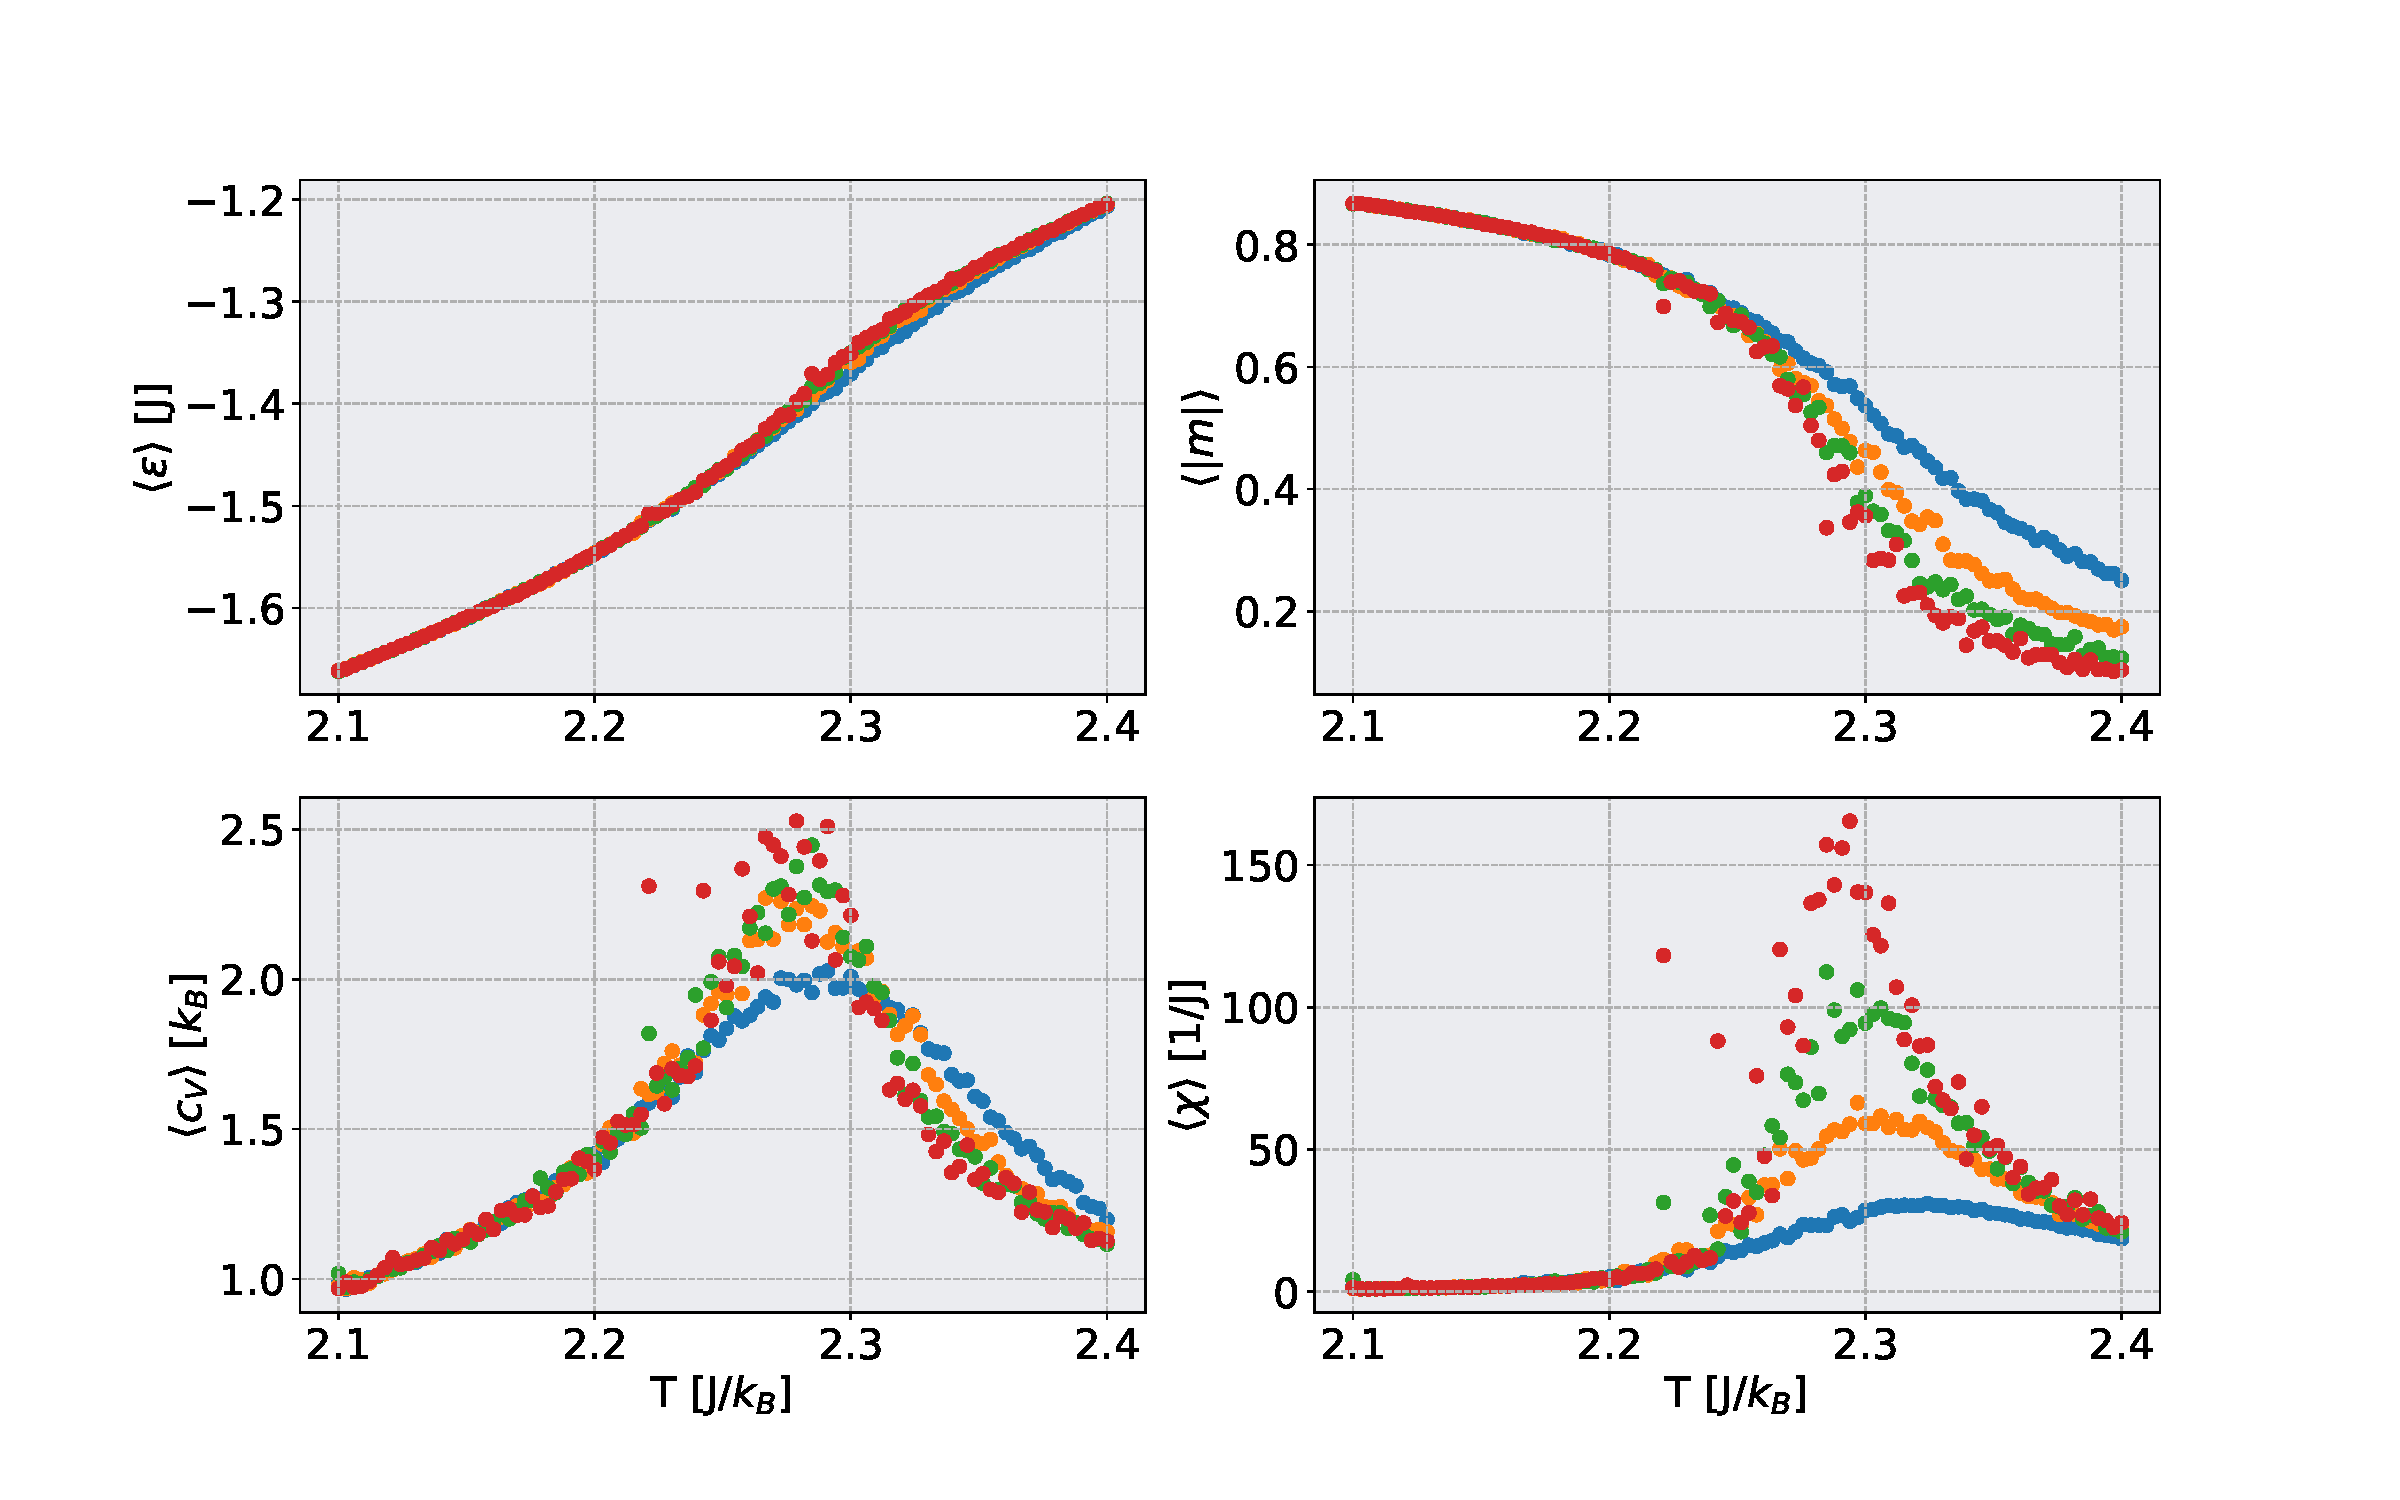
\includegraphics[scale=0.23]{figures/8.pdf} %Imports the figure.
    \caption{Blue:$L=40$, Orange:$L=60$, Green:$L=80$, Red:$L=100$. Plot shows values of interest for different lattice sizes as a function of temperature.}
    \label{fig:7}
\end{figure}


Now we need to isolate the temperature at which $c_V$ and $\chi$ are highest. This turns out not to be easy, as the resolution around these sections is poor. The sections seem to be nicer for $\chi$, so this is the variable we will use. Instead of simply finding the highest variable for each lattice, we will calculate the average energy for the five highest points. Afterward, we run a linear regression to find the intercept for the regression as $L=\infty \Rightarrow 1/L = 0$. A plot of this is provided in figure \ref{fig:8}. The estimate for the critical temperature on an infinite lattice is $T_C = 2.273 \pm 0.008 k_B$, where the correct value is $\approx 2.296 J/k_B$. In the uncertainties there is included both the standard division from the graph and the uncertainty associated with linear regression.


\begin{figure}[h!]
    \centering %Centers the figure
    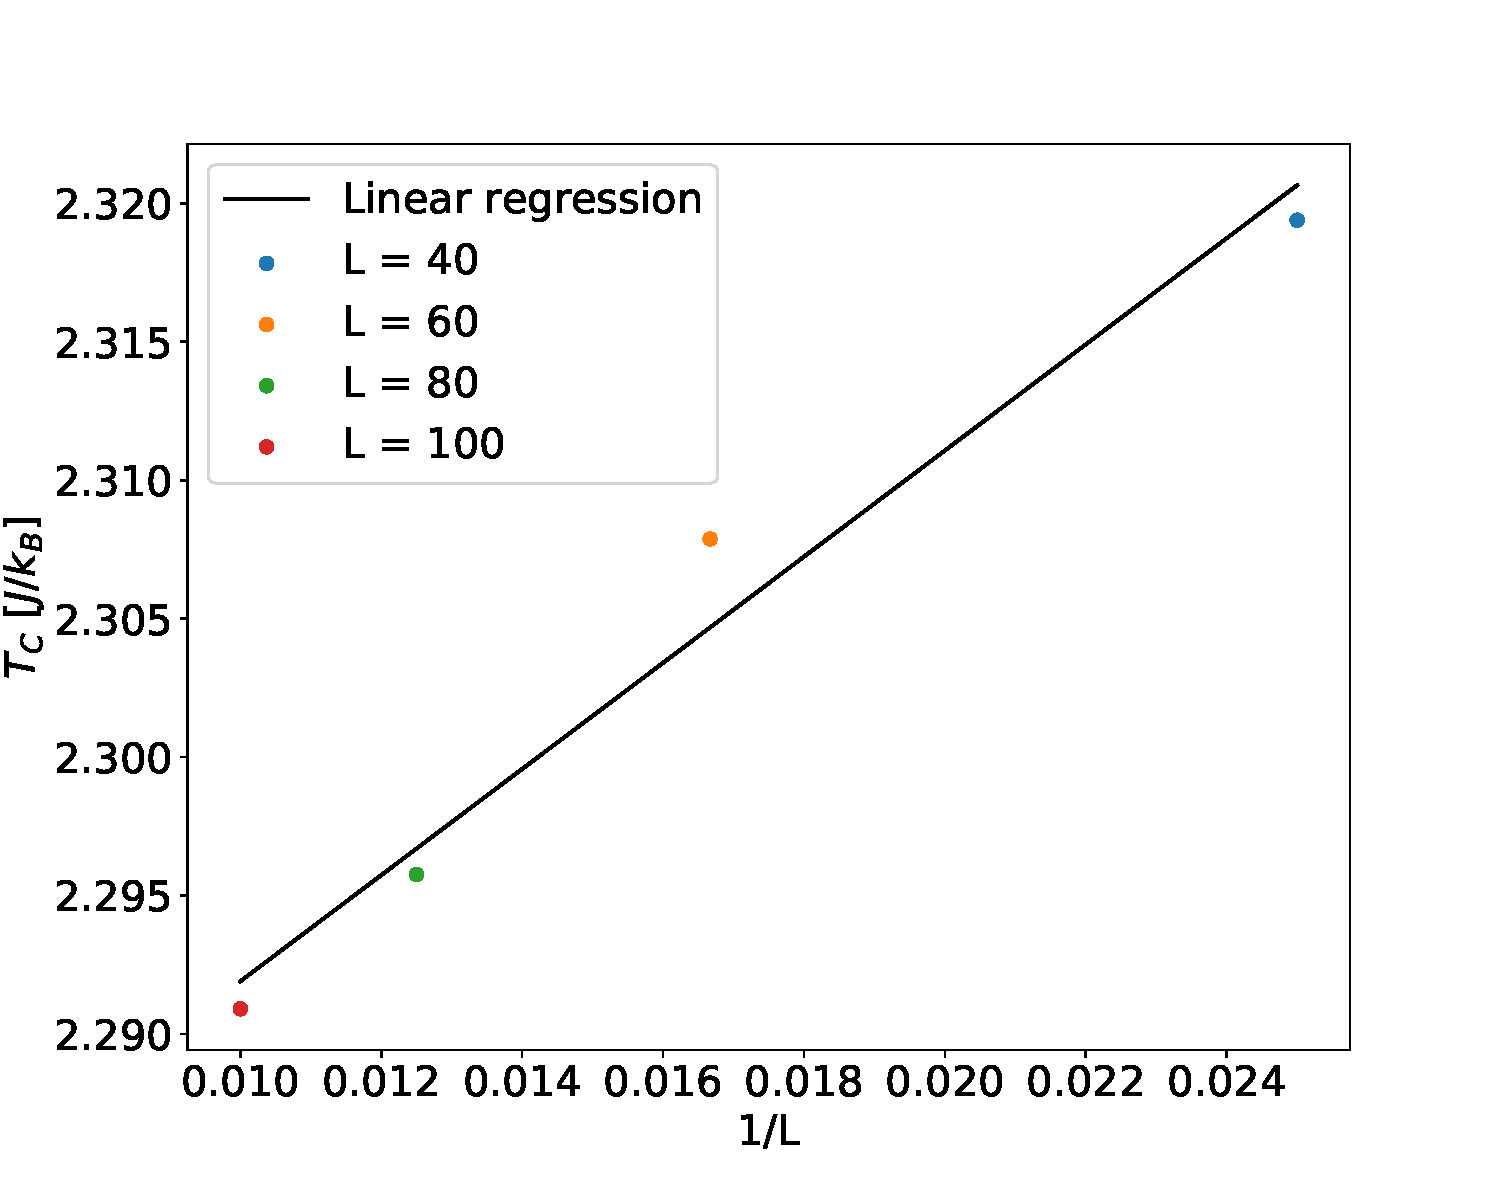
\includegraphics[scale=0.35]{figures/9.pdf} %Imports the figure.
    \caption{Plot shows a numerical estimate of critical temperature $T_C$ as a function of lattice size $L$ and their linear regression.}
    \label{fig:8}
\end{figure}
\FloatBarrier






% ===========================================
\section{Conclusion}\label{sec:conclusion}
We have computed the evolution of a finite 2D Ising model with periodic boundary conditions using the Marco chain Monte Carlo method and the Metropolis algorithm. We found some estimates for statistical uncertainty and burn-in time on a 2x2 and 20x20 lattice respectively, which showed to be on the order of $10^3$ MC cycles. We compared the analytical solutions for a two-by-two lattice, with the numerical result using $10^6$ steps, We managed to validate our implementation and algorithm. We sampled a pmf, which acted really intuitively, and for temperatures higher than critical it showed to have a close-to-normal distribution. Finally, we managed to determine the critical temperature of an infinite lattice with an uncertainty of $\pm 0.008 [J/k_b]$, which is almost surprisingly close to Onsager's original value.


% ===========================================

\section{References}
[1] Computational Physics compendium by  Morten Hjorth-Jensen, Department of Physics, University of Oslo

URL to GitHub repo:
\url{https://github.uio.no/lukasce/FYS3150_Project_4.git}

\end{document}


